\documentclass[a4paper]{article}
\renewcommand{\epsilon}{\varepsilon}
\newcommand{\triposcourse}{Linear Algebra}
\usepackage{fancyhdr,titlesec,geometry}
\usepackage[dvipsnames]{xcolor}
\usepackage[many]{tcolorbox}
\usepackage{xifthen}
\usepackage{import}
\usepackage{parskip}
\usepackage{transparent}
\usepackage{mathtools,amssymb,amsfonts,amsthm,bm}   % Math Presets
\usepackage{array,tabularx,booktabs}                % Table Presets
\usepackage{graphicx,wrapfig,float,caption}         % Figure Presets
\usepackage{setspace,multicol}                      % Text Presets
\usepackage{tikz,physics,cancel,tkz-euclide,pgfplots,tikz-3dplot}                    % Physics Presets
\usepackage{amsmath}
\usepackage{mathrsfs}
\usepackage{enumerate}
\usepackage[shortlabels]{enumitem}
\usepackage{hyperref}
\usepackage{lipsum}
\usepackage{IEEEtrantools}
\usepackage{xcomment}
\usepackage{sectsty}
\usepackage{thmtools}
\usepackage{mdframed}
\usepackage{siunitx}
\usepackage{centernot}

\newcommand{\sectionbreak}{\clearpage}

\tdplotsetmaincoords{60}{120}

\usetikzlibrary{arrows.meta}
\usetikzlibrary{decorations.markings}
\usetikzlibrary{decorations.pathmorphing}
\usetikzlibrary{automata, positioning}
\usetikzlibrary{fadings}
\usetikzlibrary{intersections}
\usetikzlibrary{cd}
\usetikzlibrary{patterns}
\usetikzlibrary{shapes.arrows}
\usepgfplotslibrary{colormaps, external}
\pgfarrowsdeclarecombine{twolatex'}{twolatex'}{latex'}{latex'}{latex'}{latex'}
\tikzset{->/.style = {decoration={markings,
                                  mark=at position 1 with {\arrow[scale=1.6]{latex'}}},
                      postaction={decorate}}}
\tikzset{<-/.style = {decoration={markings,
                                  mark=at position 0 with {\arrowreversed[scale=1.6]{latex'}}},
                      postaction={decorate}}}
\tikzset{<->/.style = {decoration={markings,
                                   mark=at position 0 with {\arrowreversed[scale=1.6]{latex'}},
                                   mark=at position 1 with {\arrow[scale=1.6]{latex'}}},
                       postaction={decorate}}}
\tikzset{->-/.style = {decoration={markings,
                                   mark=at position #1 with {\arrow[scale=1.6]{latex'}}},
                       postaction={decorate}}}
\tikzset{-<-/.style = {decoration={markings,
                                   mark=at position #1 with {\arrowreversed[scale=1.6]{latex'}}},
                       postaction={decorate}}}
\tikzset{->>/.style = {decoration={markings,
                                  mark=at position 1 with {\arrow[scale=1.6]{twolatex'}}},
                      postaction={decorate}}}
\tikzset{<<-/.style = {decoration={markings,
                                  mark=at position 0 with {\arrowreversed[scale=1.6]{twolatex'}}},
                      postaction={decorate}}}
\tikzset{<<->>/.style = {decoration={markings,
                                   mark=at position 0 with {\arrowreversed[scale=1.6]{twolatex'}},
                                   mark=at position 1 with {\arrow[scale=1.6]{twolatex'}}},
                       postaction={decorate}}}
\tikzset{->>-/.style = {decoration={markings,
                                   mark=at position #1 with {\arrow[scale=1.6]{twolatex'}}},
                       postaction={decorate}}}
\tikzset{-<<-/.style = {decoration={markings,
                                   mark=at position #1 with {\arrowreversed[scale=1.6]{twolatex'}}},
                       postaction={decorate}}}

\tikzset{
set arrow inside/.code={\pgfqkeys{/tikz/arrow inside}{#1}},
set arrow inside={end/.initial=>, opt/.initial=},
/pgf/decoration/Mark/.style={
    mark/.expanded=at position #1 with
    {
        \noexpand\arrow[\pgfkeysvalueof{/tikz/arrow inside/opt}]{\pgfkeysvalueof{/tikz/arrow inside/end}}
    }
},
arrow inside/.style 2 args={
    set arrow inside={#1},
    postaction={
        decorate,decoration={
            markings,Mark/.list={#2}
        }
    }
},
}

\tikzstyle{circ}=[fill=black, draw=black, shape=circle]
\tikzset{
dot/.style = {circle, fill, minimum size=#1,
              inner sep=0pt, outer sep=0pt},
dot/.default = 5pt% size of the circle diameter 
}
\tikzset{mstate/.style={circle, draw, blue, text=black, minimum width=0.7cm}}
\tikzset{snake it/.style={-stealth,
decoration={snake, 
    amplitude = .4mm,
    segment length = 2mm,
    post length=0.9mm},decorate}}

\def\centerarc[#1](#2)(#3:#4:#5)% Syntax: [draw options](center)(initial angle:final angle:radius)
    { \draw[#1] ($(#2)+({#5*cos(#3)},{#5*sin(#3)})$) arc (#3:#4:#5); }

\hypersetup{
    colorlinks=true,
    linkcolor=blue,
    filecolor=blue,
    citecolor = black,      
    urlcolor=cyan,
    }

%%%%%%%%%%% Snippets %%%%%%%%%%%%%%%%
\newcommand*\widefbox[1]{\fbox{\hspace{2em}#1\hspace{2em}}}
\newcommand{\xint}{\int_{x_1}^{x_2}}
\newcommand{\mw}{\sqrt{m\omega}}
\newcommand{\de}{\delta}
\newcommand{\dde}{\dot{\delta}}
\newcommand{\di}{\delta_i}
\newcommand{\ddi}{\dot{\delta_i}}
\newcommand{\dddi}{\ddot{\delta_i}}
\newcommand{\dipl}{\delta_{i+1}}
\newcommand{\dimi}{\delta_{i-1}}
\newcommand{\ddt}[1]{\frac{{d} #1}{dt}}
\newcommand{\ddtt}[1]{\frac{d^2 #1}{dt^2}}
\newcommand{\ddx}[1]{\frac{d #1}{dx}}
\newcommand{\ddxx}[1]{\frac{d^2 #1}{dx^2}}
\newcommand{\eps}{\epsilon}
\newcommand{\del}[2]{\frac{\partial #1}{\partial #2}}
\newcommand{\deltwo}[2]{\frac{\partial^2 #1}{\partial #2^2}}
\newcommand{\lam}{\lambda}
\newcommand{\Lam}{\Lambda}
\newcommand{\sig}{\sigma}
\newcommand{\Sig}{\Sigma}
\newcommand{\half}{\frac{1}{2}}
\newcommand{\munu}{{\mu\nu}}
\newcommand{\thalf}{\tfrac{1}{2}}
\renewcommand{\div}{\nabla\cdot}
\renewcommand{\curl}{\nabla\times}

\DeclareMathOperator{\orb}{Orb}
\DeclareMathOperator{\stab}{Stab}
\DeclareMathOperator{\adj}{adj}
\DeclareMathOperator{\ccl}{ccl}
\let\var\relax
\DeclareMathOperator{\var}{Var}
\DeclareMathOperator{\cov}{Cov}
\DeclareMathOperator{\corr}{Corr}
\DeclareMathOperator{\Markov}{Markov}
\DeclareMathOperator{\nullity}{nullity}

\newcommand{\bfA}{{\bf A}}
\newcommand{\bfB}{{\bf B}}
\newcommand{\bfC}{{\bf C}}
\newcommand{\bfD}{{\bf D}}
\newcommand{\bfE}{{\bf E}}
\newcommand{\bfF}{{\bf F}}
\newcommand{\bfG}{{\bf G}}
\newcommand{\bfH}{{\bf H}}
\newcommand{\bfI}{{\bf I}}
\newcommand{\bfJ}{{\bf J}}
\newcommand{\bfK}{{\bf K}}
\newcommand{\bfL}{{\bf L}}
\newcommand{\bfM}{{\bf M}}
\newcommand{\bfN}{{\bf N}}
\newcommand{\bfO}{{\bf O}}
\newcommand{\bfP}{{\bf P}}
\newcommand{\bfQ}{{\bf Q}}
\newcommand{\bfR}{{\bf R}}
\newcommand{\bfS}{{\bf S}}
\newcommand{\bfT}{{\bf T}}
\newcommand{\bfU}{{\bf U}}
\newcommand{\bfV}{{\bf V}}
\newcommand{\bfW}{{\bf W}}
\newcommand{\bfX}{{\bf X}}
\newcommand{\bfY}{{\bf Y}}
\newcommand{\bfZ}{{\bf Z}}

\newcommand{\bfa}{{\bf a}}
\newcommand{\bfb}{{\bf b}}
\newcommand{\bfc}{{\bf c}}
\newcommand{\bfd}{{\bf d}}
\newcommand{\bfe}{{\bf e}}
\newcommand{\bff}{{\bf f}}
\newcommand{\bfg}{{\bf g}}
\newcommand{\bfh}{{\bf h}}
\newcommand{\bfi}{{\bf i}}
\newcommand{\bfj}{{\bf j}}
\newcommand{\bfk}{{\bf k}}
\newcommand{\bfl}{{\bf l}}
\newcommand{\bfm}{{\bf m}}
\newcommand{\bfn}{{\bf n}}
\newcommand{\bfo}{{\bf o}}
\newcommand{\bfp}{{\bf p}}
\newcommand{\bfq}{{\bf q}}
\newcommand{\bfr}{{\bf r}}
\newcommand{\bfs}{{\bf s}}
\newcommand{\bft}{{\bf t}}
\newcommand{\bfu}{{\bf u}}
\newcommand{\bfv}{{\bf v}}
\newcommand{\bfw}{{\bf w}}
\newcommand{\bfx}{{\bf x}}
\newcommand{\bfy}{{\bf y}}
\newcommand{\bfz}{{\bf z}}

\newcommand{\mcA}{{\mathcal{A}}}
\newcommand{\mcB}{{\mathcal{B}}}
\newcommand{\mcC}{{\mathcal{C}}}
\newcommand{\mcD}{{\mathcal{D}}}
\newcommand{\mcE}{{\mathcal{E}}}
\newcommand{\mcF}{{\mathcal{F}}}
\newcommand{\mcG}{{\mathcal{G}}}
\newcommand{\mcH}{{\mathcal{H}}}
\newcommand{\mcI}{{\mathcal{I}}}
\newcommand{\mcJ}{{\mathcal{J}}}
\newcommand{\mcK}{{\mathcal{K}}}
\newcommand{\mcL}{{\mathcal{L}}}
\newcommand{\mcM}{{\mathcal{M}}}
\newcommand{\mcN}{{\mathcal{N}}}
\newcommand{\mcO}{{\mathcal{O}}}
\newcommand{\mcP}{{\mathcal{P}}}
\newcommand{\mcQ}{{\mathcal{Q}}}
\newcommand{\mcR}{{\mathcal{R}}}
\newcommand{\mcS}{{\mathcal{S}}}
\newcommand{\mcT}{{\mathcal{T}}}
\newcommand{\mcU}{{\mathcal{U}}}
\newcommand{\mcV}{{\mathcal{V}}}
\newcommand{\mcW}{{\mathcal{W}}}
\newcommand{\mcX}{{\mathcal{X}}}
\newcommand{\mcY}{{\mathcal{Y}}}
\newcommand{\mcZ}{{\mathcal{Z}}}

\newcommand{\bbA}{{\mathbb{A}}}
\newcommand{\bbB}{{\mathbb{B}}}
\newcommand{\bbC}{{\mathbb{C}}}
\newcommand{\bbD}{{\mathbb{D}}}
\newcommand{\bbE}{{\mathbb{E}}}
\newcommand{\bbF}{{\mathbb{F}}}
\newcommand{\bbG}{{\mathbb{G}}}
\newcommand{\bbH}{{\mathbb{H}}}
\newcommand{\bbI}{{\mathbb{I}}}
\newcommand{\bbJ}{{\mathbb{J}}}
\newcommand{\bbK}{{\mathbb{K}}}
\newcommand{\bbL}{{\mathbb{L}}}
\newcommand{\bbM}{{\mathbb{M}}}
\newcommand{\bbN}{{\mathbb{N}}}
\newcommand{\bbO}{{\mathbb{O}}}
\newcommand{\bbP}{{\mathbb{P}}}
\newcommand{\bbQ}{{\mathbb{Q}}}
\newcommand{\bbR}{{\mathbb{R}}}
\newcommand{\bbS}{{\mathbb{S}}}
\newcommand{\bbT}{{\mathbb{T}}}
\newcommand{\bbU}{{\mathbb{U}}}
\newcommand{\bbV}{{\mathbb{V}}}
\newcommand{\bbW}{{\mathbb{W}}}
\newcommand{\bbX}{{\mathbb{X}}}
\newcommand{\bbY}{{\mathbb{Y}}}
\newcommand{\bbZ}{{\mathbb{Z}}}

\newcommand{\mfa}{{\mathfrak{a}}}
\newcommand{\mfb}{{\mathfrak{b}}}
\newcommand{\mfc}{{\mathfrak{c}}}
\newcommand{\mfd}{{\mathfrak{d}}}
\newcommand{\mfe}{{\mathfrak{e}}}
\newcommand{\mff}{{\mathfrak{f}}}
\newcommand{\mfg}{{\mathfrak{g}}}
\newcommand{\mfh}{{\mathfrak{h}}}
\newcommand{\mfi}{{\mathfrak{i}}}
\newcommand{\mfj}{{\mathfrak{j}}}
\newcommand{\mfk}{{\mathfrak{k}}}
\newcommand{\mfl}{{\mathfrak{l}}}
\newcommand{\mfm}{{\mathfrak{m}}}
\newcommand{\mfn}{{\mathfrak{n}}}
\newcommand{\mfo}{{\mathfrak{o}}}
\newcommand{\mfp}{{\mathfrak{p}}}
\newcommand{\mfq}{{\mathfrak{q}}}
\newcommand{\mfr}{{\mathfrak{r}}}
\newcommand{\mfs}{{\mathfrak{s}}}
\newcommand{\mft}{{\mathfrak{t}}}
\newcommand{\mfu}{{\mathfrak{u}}}
\newcommand{\mfv}{{\mathfrak{v}}}
\newcommand{\mfw}{{\mathfrak{w}}}
\newcommand{\mfx}{{\mathfrak{x}}}
\newcommand{\mfy}{{\mathfrak{y}}}
\newcommand{\mfz}{{\mathfrak{z}}}

\newcommand{\mfA}{{\mathfrak{A}}}
\newcommand{\mfB}{{\mathfrak{B}}}
\newcommand{\mfC}{{\mathfrak{C}}}
\newcommand{\mfD}{{\mathfrak{D}}}
\newcommand{\mfE}{{\mathfrak{E}}}
\newcommand{\mfF}{{\mathfrak{F}}}
\newcommand{\mfG}{{\mathfrak{G}}}
\newcommand{\mfH}{{\mathfrak{H}}}
\newcommand{\mfI}{{\mathfrak{I}}}
\newcommand{\mfJ}{{\mathfrak{J}}}
\newcommand{\mfK}{{\mathfrak{K}}}
\newcommand{\mfL}{{\mathfrak{L}}}
\newcommand{\mfM}{{\mathfrak{M}}}
\newcommand{\mfN}{{\mathfrak{N}}}
\newcommand{\mfO}{{\mathfrak{O}}}
\newcommand{\mfP}{{\mathfrak{P}}}
\newcommand{\mfQ}{{\mathfrak{Q}}}
\newcommand{\mfR}{{\mathfrak{R}}}
\newcommand{\mfS}{{\mathfrak{S}}}
\newcommand{\mfT}{{\mathfrak{T}}}
\newcommand{\mfU}{{\mathfrak{U}}}
\newcommand{\mfV}{{\mathfrak{V}}}
\newcommand{\mfW}{{\mathfrak{W}}}
\newcommand{\mfX}{{\mathfrak{X}}}
\newcommand{\mfY}{{\mathfrak{Y}}}
\newcommand{\mfZ}{{\mathfrak{Z}}}

\newcommand{\rma}{\mathrm{a}}
\newcommand{\rmb}{\mathrm{b}}
\newcommand{\rmc}{\mathrm{c}}
\newcommand{\rmd}{\mathrm{d}}
\renewcommand{\dd}{\,\mathrm{d}}
\newcommand{\rme}{\mathrm{e}}
\newcommand{\rmf}{\mathrm{f}}
\newcommand{\rmg}{\mathrm{g}}
\newcommand{\rmh}{\mathrm{h}}
\newcommand{\rmi}{\mathrm{i}}
\newcommand{\rmj}{\mathrm{j}}
\newcommand{\rmk}{\mathrm{k}}
\newcommand{\rml}{\mathrm{l}}
\newcommand{\rmm}{\mathrm{m}}
\newcommand{\rmn}{\mathrm{n}}
\newcommand{\rmo}{\mathrm{o}}
\newcommand{\rmp}{\mathrm{p}}
\newcommand{\rmq}{\mathrm{q}}
\newcommand{\rmr}{\mathrm{r}}
\newcommand{\rms}{\mathrm{s}}
\newcommand{\rmt}{\mathrm{t}}
\newcommand{\rmu}{\mathrm{u}}
\newcommand{\rmv}{\mathrm{v}}
\newcommand{\rmw}{\mathrm{w}}
\newcommand{\rmx}{\mathrm{x}}
\newcommand{\rmy}{\mathrm{y}}
\newcommand{\rmz}{\mathrm{z}}
\newcommand{\rmA}{\mathrm{A}}
\newcommand{\rmB}{\mathrm{B}}
\newcommand{\rmC}{\mathrm{C}}
\newcommand{\rmD}{\mathrm{D}}
\newcommand{\rmE}{\mathrm{E}}
\newcommand{\rmF}{\mathrm{F}}
\newcommand{\rmG}{\mathrm{G}}
\newcommand{\rmH}{\mathrm{H}}
\newcommand{\rmI}{\mathrm{I}}
\newcommand{\rmJ}{\mathrm{J}}
\newcommand{\rmK}{\mathrm{K}}
\newcommand{\rmL}{\mathrm{L}}
\newcommand{\rmM}{\mathrm{M}}
\newcommand{\rmN}{\mathrm{N}}
\newcommand{\rmO}{\mathrm{O}}
\newcommand{\rmP}{\mathrm{P}}
\newcommand{\rmQ}{\mathrm{Q}}
\newcommand{\rmR}{\mathrm{R}}
\newcommand{\rmS}{\mathrm{S}}
\newcommand{\rmT}{\mathrm{T}}
\newcommand{\rmU}{\mathrm{U}}
\newcommand{\rmV}{\mathrm{V}}
\newcommand{\rmW}{\mathrm{W}}
\newcommand{\rmX}{\mathrm{X}}
\newcommand{\rmY}{\mathrm{Y}}
\newcommand{\rmZ}{\mathrm{Z}}

\newcommand{\GL}{\mathrm{GL}}
\newcommand{\Or}{\mathrm{O}}
\newcommand{\PGL}{\mathrm{PGL}}
\newcommand{\PSL}{\mathrm{PSL}}
\newcommand{\PSO}{\mathrm{PSO}}
\newcommand{\PSU}{\mathrm{PSU}}
\newcommand{\SL}{\mathrm{SL}}
\newcommand{\SO}{\mathrm{SO}}
\newcommand{\Spin}{\mathrm{Spin}}
\newcommand{\Sp}{\mathrm{Sp}}
\newcommand{\SU}{\mathrm{SU}}
\newcommand{\Mat}{\mathrm{Mat}}

% Some common notations

\renewcommand{\v}{\mathbf{v}}
\newcommand{\w}{\mathbf{w}}
\renewcommand{\u}{\mathbf{u}}

% Matrix algebras
\newcommand{\gl}{\mathfrak{gl}}
\newcommand{\ort}{\mathfrak{o}}
\newcommand{\so}{\mathfrak{so}}
\newcommand{\su}{\mathfrak{su}}
\newcommand{\uu}{\mathfrak{u}}
\renewcommand{\sl}{\mathfrak{sl}}
\newcommand{\inner}[1]{\left\langle{#1}\right\rangle}
\DeclareMathOperator{\spn}{span}

\newcommand{\mobius}{{M\"{o}bius }}

\renewcommand{\ge}{\geqslant}
\renewcommand{\le}{\leqslant}
\renewcommand{\geq}{\geqslant}
\renewcommand{\leq}{\leqslant}
\renewcommand{\restriction}{\mathord{\upharpoonright}}

\newcommand\independent{\protect\mathpalette{\protect\independenT}{\perp}}
\def\independenT#1#2{\mathrel{\rlap{$#1#2$}\mkern2mu{#1#2}}}

\setlength{\parindent}{0pt}
% \setlength{\parskip}{\baselineskip}
\newcommand{\incfig}[1]{%
    \def\svgwidth{0.4\columnwidth}
    \import{./figures/}{#1.pdf_tex}
}
%%%%%%%%%%%%%%%%%%%%%%%%%%%%%%%%%%%%%

\usepackage[T1]{fontenc}
\usepackage{lmodern,mathrsfs}

%%%%%%%boxed enviroment for final layout%%%%%%%%%%%%%

\newtheoremstyle{mystyle}%
  {}%
  {}%
  {}%
  {}%
  {\sffamily\bfseries}%
  {.}%
  { }%
  {}%

% \renewenvironment{proof}{{\sffamily\bfseries Proof. }}{\qed}

\theoremstyle{mystyle}{
  \newtheorem{theorem}{Theorem}[section]
  \newtheorem{lemma}[theorem]{Lemma}
  \newtheorem{proposition}[theorem]{Proposition}
  \newtheorem{corollary}[theorem]{Corollary}
  \newtheorem{problem}[theorem]{Problem}
  \newtheorem*{claim}{Claim}
  \newtheorem*{slemma}{Lemma}
  \newtheorem*{sprop}{Proposition}
  \newtheorem*{notation}{Notation}

  \newtheorem{inquestion}{Question}
  \newtheorem*{sque}{Question}

  \newtheorem{definition}{Definition}[section]
  \newtheorem{conjecture}{Conjecture}[section]
  \newtheorem{example}{Example}[section]
  \newtheorem*{law}{Law}

  \newtheorem*{remark}{Remark}
  \newtheorem*{note}{Note}
}

\newenvironment{question}[1]
{\renewcommand\theinquestion{#1}\inquestion}
{\endinquestion}

\theoremstyle{definition}{
    \newtheorem*{exercise}{Exercise}}

\tcolorboxenvironment{definition}{
  boxrule=0pt,
  boxsep=2pt,
  colback={White!90!Cerulean},
  enhanced jigsaw, 
  borderline west={2pt}{0pt}{Cerulean},
  sharp corners,
  before skip=10pt,
  after skip=10pt,
  breakable,
  % parbox=false,
}

\tcolorboxenvironment{notation}{
  boxrule=0pt,
  boxsep=2pt,
  colback={White!90!Cerulean},
  enhanced jigsaw, 
  borderline west={2pt}{0pt}{Cerulean},
  sharp corners,
  before skip=10pt,
  after skip=10pt,
  breakable,
  % parbox=false,
}

\tcolorboxenvironment{proposition}{
  boxrule=0pt,
  boxsep=2pt,
  colback={White!90!Yellow},
  enhanced jigsaw, 
  borderline west={2pt}{0pt}{Yellow},
  sharp corners,
  before skip=10pt,
  after skip=10pt,
  breakable,
  % parbox=false,
}

\tcolorboxenvironment{sprop}{
  boxrule=0pt,
  boxsep=2pt,
  colback={White!90!Yellow},
  enhanced jigsaw, 
  borderline west={2pt}{0pt}{Yellow},
  sharp corners,
  before skip=10pt,
  after skip=10pt,
  breakable,
  % parbox=false,
}

\tcolorboxenvironment{theorem}{
  boxrule=0pt,
  boxsep=2pt,
  colback={White!90!Dandelion},
  enhanced jigsaw, 
  borderline west={2pt}{0pt}{Dandelion},
  sharp corners,
  before skip=10pt,
  after skip=10pt,
  breakable,
  % parbox=false,
}

\tcolorboxenvironment{lemma}{
  boxrule=0pt,
  boxsep=2pt,
  blanker,
  borderline west={2pt}{0pt}{Red},
  before skip=10pt,
  after skip=10pt,
  sharp corners,
  left=12pt,
  right=12pt,
  breakable,
  % parbox=false,
}

\tcolorboxenvironment{corollary}{
  boxrule=0pt,
  boxsep=2pt,
  blanker,
  borderline west={2pt}{0pt}{ForestGreen},
  before skip=10pt,
  after skip=10pt,
  sharp corners,
  left=12pt,
  right=12pt,
  breakable,
  % parbox=false,
}

\tcolorboxenvironment{proof}{
  boxrule=0pt,
  boxsep=2pt,
  blanker,
  borderline west={2pt}{0pt}{NavyBlue!80!white},
  before skip=10pt,
  after skip=10pt,
  left=12pt,
  right=12pt,
  breakable,
  % parbox=false,
}

\tcolorboxenvironment{remark}{
  boxrule=0pt,
  boxsep=2pt,
  blanker,
  borderline west={2pt}{0pt}{Green},
  before skip=10pt,
  after skip=10pt,
  left=12pt,
  right=12pt,
  breakable,
  % parbox=false,
}

\tcolorboxenvironment{note}{
  boxrule=0pt,
  boxsep=2pt,
  blanker,
  borderline west={2pt}{0pt}{PineGreen},
  before skip=10pt,
  after skip=10pt,
  left=12pt,
  right=12pt,
  breakable,
  % parbox=false,
}

\tcolorboxenvironment{example}{
  boxrule=0pt,
  boxsep=2pt,
  blanker,
  borderline west={2pt}{0pt}{Black},
  sharp corners,
  before skip=10pt,
  after skip=10pt,
  left=12pt,
  right=12pt,
  breakable,
  % parbox=false,
}

\titleformat*{\section}{\Large\bfseries\sffamily}
\titleformat*{\subsection}{\large\bfseries\sffamily}
\titleformat*{\subsubsection}{\bfseries\sffamily}
\titleformat*{\paragraph}{\bfseries\sffamily}

%%%%%%%%%%%%%%%%%%%%%%%%%%%%%%%%%%%%%%%%%%%%%%%%%%%%

\title{\textbf{\sffamily\triposcourse{} Notes}}
% \usepackage[T1]{fontenc}
\usepackage{crimson}

\theoremstyle{plain}

\theoremstyle{definition}
\newtheorem{theorem}{Theorem}[section]
\newtheorem{lemma}[theorem]{Lemma}
\newtheorem{proposition}[theorem]{Proposition}
\newtheorem{corollary}[theorem]{Corollary}
\newtheorem{problem}[theorem]{Problem}
\newtheorem*{claim}{Claim}
\newtheorem*{slemma}{Lemma}
\newtheorem*{sprop}{Proposition}
\newtheorem*{notation}{Notation}
\newtheorem*{exercise}{Exercise}

\newtheorem{inquestion}{Question}
\newtheorem*{sque}{Question}
\newenvironment{question}[1]
  {\renewcommand\theinquestion{#1}\inquestion}
  {\endinquestion}

\newtheorem{definition}{Definition}[section]
\newtheorem{conjecture}{Conjecture}[section]
\newtheorem{example}{Example}[section]
\newtheorem*{law}{Law}

\theoremstyle{remark}
\newtheorem*{remark}{Remark}
\newtheorem*{note}{Note}

\title{\textbf{\triposcourse{} Notes}}
% \theoremstyle{plain}{
  \newtheorem{theorem}{Theorem}[section]
  \newtheorem{lemma}[theorem]{Lemma}
  \newtheorem{proposition}[theorem]{Proposition}
  \newtheorem{corollary}[theorem]{Corollary}
  \newtheorem*{claim}{Claim}
  \newtheorem*{slemma}{Lemma}
  \newtheorem*{sprop}{Proposition}
  \newtheorem{conjecture}{Conjecture}[section]
  \newtheorem*{law}{Law}
  \newtheorem{inquestion}{Question}
  \newtheorem*{sque}{Question}
}

\theoremstyle{definition}{
  \newtheorem{method}[theorem]{Method}
  \newtheorem{definition}{Definition}[section]
  \newtheorem{example}{Example}[section]
  \newtheorem*{notation}{Notation}
  \newtheorem*{exercise}{Exercise}
}

\theoremstyle{remark}{
  \newtheorem{remark}[theorem]{Remark}
  \newtheorem*{note}{Note}
}

\newenvironment{question}[1]
{\renewcommand\theinquestion{#1}\inquestion}
{\endinquestion}

\title{\textbf{\sffamily\triposcourse{} Notes}}

%layout full
% \geometry{%
%   a4paper,
%   lmargin=2cm,
%   rmargin=2.5cm,
%   tmargin=3.5cm,
%   bmargin=2.5cm,
%   footskip=12pt,
%   headheight=24pt}
% layout trim
% \geometry{
% papersize={379pt, 542pt},
% textwidth=345pt,
% textheight=443pt,
% left=17pt,
% top=54pt,
% right=17pt
% }
% layout a5
\geometry{%
  a5paper,
  lmargin=1cm,
  rmargin=1cm,
  tmargin=2.5cm,
  bmargin=1.5cm,
  footskip=15pt,
  headheight=24pt}
\pagestyle{fancy}
\rhead{{\triposcourse{}}}
\author{jt775}
\AddToHook{cmd/section/before}{\clearpage}

\graphicspath{ {./images/} }
\pgfplotsset{compat=1.17}
\begin{document}
\maketitle
\tableofcontents
\newpage
\part*{Lecture 1}
\section{Vector Spaces}
\subsection{Vector spaces and subspaces}
Let $ \bbF $ be an arbitrary field ($ \mathbb{R}  $ or $ \mathbb{C}  $).

\begin{definition}[$ \bbF $ Vector Space]
    An \textit{$ \bbF$ vector space} (or a \textit{vector space over $\bbF$}) is a an abelian group $ (V,+) $ with a function $ \bbF\times V \mapsto V $, defined by $ (\lambda, \bfv) \mapsto \lambda\bfv $, such that 
    \begin{enumerate}
        \item $ \lambda(\bfv_1+\bfv_2)=\lambda\bfv_1+\lambda\bfv_2 $,
        \item $ (\lambda_1+\lambda_2)\bfv = \lambda_1\bfv+\lambda_2\bfv $,
        \item $ \lambda(\mu\bfv)=(\lambda\mu)\bfv $,
        \item $ 1\bfv=\bfv $,
    \end{enumerate}
    for all $ \lambda,\mu\in \bbF$ and $ \bfv\in V $.
\end{definition}

\begin{example}
    \begin{enumerate}
        \item $ \bbF^n,\ n\in \mathbb{N}  $ is a vector space.
        \item $ \bbR^X $, where $X$ is a set, is a vector space.
        \item $ \mcM_{n,m}(\bbF) $ is a vector space.
    \end{enumerate}
\end{example}
\begin{remark}
    The axioms imply that $ \forall \bfv\in V,\ 0\cdot\bfv=0 $.
\end{remark}

\begin{definition}[Subspace]
    Let $V$ be a vector space on $\bbF$. A subset $U$ of $V$ is a \textit{vector subspace} if 
    \begin{enumerate}
        \item $ \mathbf{0}\in U $,
        \item $ (\bfu_1,\bfu_2)\in U\times U \Rightarrow u_1+u_2\in U $,
        \item $ (\lambda,\bfu)\in \bbF\times U \Rightarrow \lambda\bfu\in U $.
    \end{enumerate}
    Equivalently, $U$ is a subspace of $V$ if 
    \[
        \forall (\lambda,\mu)\in \bbF\times \bbF,\ \forall (\bfu,\bfv)\in U\times U,\ \lambda\bfu+\mu\bfv\in U.
    \]
    Denote $ U\le V $.
\end{definition}
Recall from Vectors and Matrices: the two definitions are equivalent.
\begin{proposition}
    Let $ V $ be a vector space over $\bbF$. If $ U\le V $, then $U$ is a vector space over $\bbF$.
\end{proposition}
\begin{example}
    \begin{enumerate}
        \item $ \mathbb{P}(\bbR)\le \mcC(\bbR)\le \mathbb{R} ^\mathbb{R}  $.
        \item The set of vectors
        $$
        \left\{\begin{pmatrix}x_1 \\ x_2 \\ x_3\end{pmatrix} : x_1, x_2, x_3 \in \bbR, x_1 + x_2 + x_3 = t\right\}
        $$
        is a subspace of $\bbR^3$ for $t = 0$ only.
    \end{enumerate}
\end{example}
\begin{proposition}[Intersecting Subspaces]
    Let $U, W \le V$. Then $U \cap W \le V$.
\end{proposition}
\begin{proof}
    Since $0 \in U$ and $0 \in W$, we have $0 \in U \cap W$. Now if $\lambda_1, \lambda_2 \in \bbF$ and $\bfv_1, \bfv_2 \in U \cap W$, then $\lambda_1 \bfv_1 + \lambda_2 \bfv_2 \in U$ and $V$, and thus is in $U \cap V$. Thus $U \cap W \le V$.
\end{proof}
The union of two subspaces is generally \emph{not} a subspace, as it is typically not closed by addition. In fact, the union is only ever a subspace if one of the subspaces is contained in the other. 
\begin{center}
    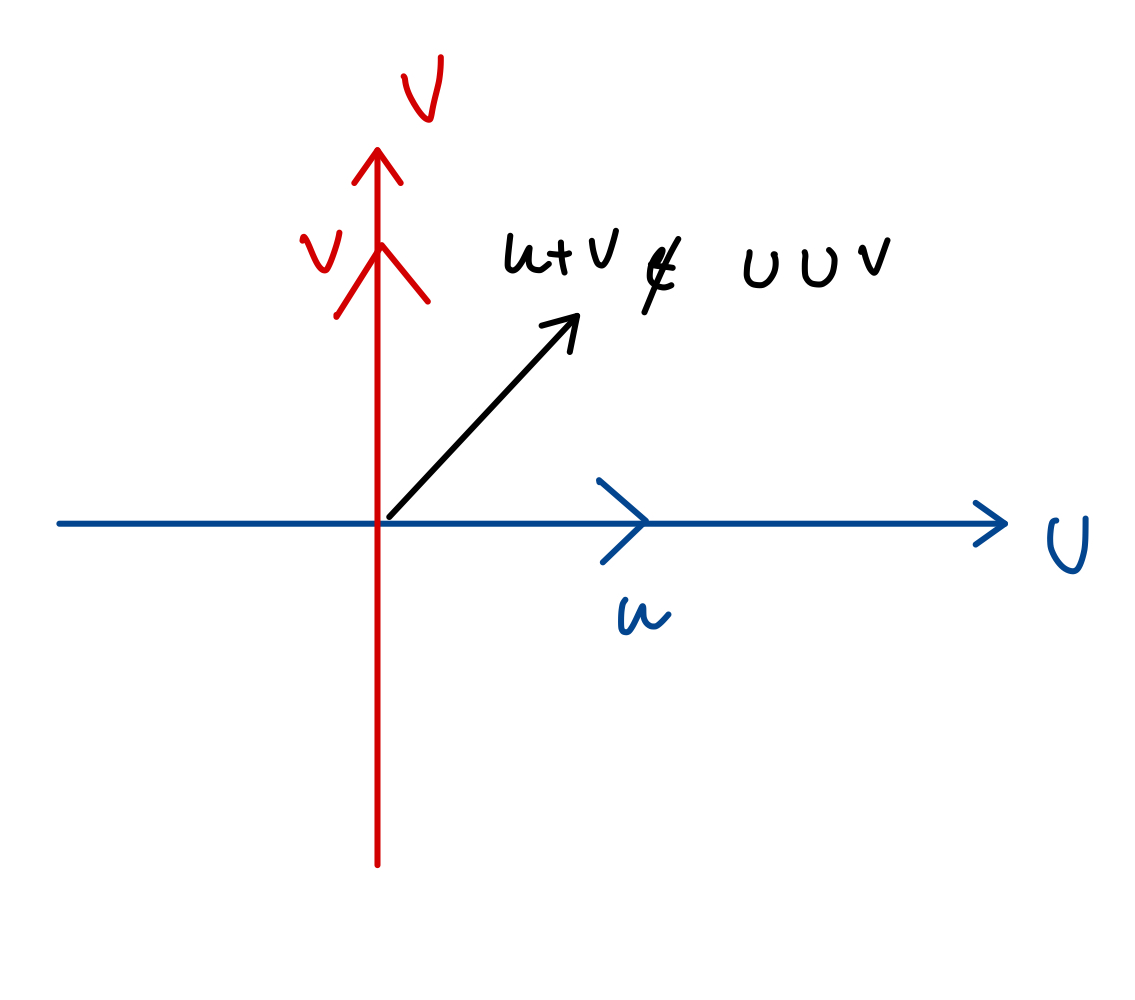
\includegraphics[scale=0.13]{la1.jpeg}
\end{center}

\begin{definition}[Sum of vector spaces]
    Let $V$ be a vector space over $\bbF$ and let $U,W\le V$. The \textit{sum} of $U,W$ is defined as 
    \[
        U+W  =\left\{ \bfu+\bfw: (\bfu,\bfw)\in U\times W \right\}.
    \] 
\end{definition}
For example, the sum of $x$-axis and $y$-axis is $ \mathbb{R}^{2} $.

\begin{proposition}
    $U+W\le V$.
\end{proposition}
\begin{proposition}
    $U+W$ is the smallest subspace of $V$ that contains $U,W$.
\end{proposition}
\begin{proof}
    Let $X$ be a subspace of $V$ that contains $U,W$. By closure, $ \bfu+\bfw\in X $ for all $ \bfu\in U,\bfw\in W $, so $ U+W\le X $. Hence it is the smallest subspace.
\end{proof}
\subsection{Subspaces and quotient}
\begin{definition}[Quotient]
    Let $V$ a vector space over $\bbF$, and let $U \leq V$. The \emph{quotient space} $V/U$ is the abelian group $V/U$ equipped with the scalar multiplication $\bbF \times V/U \rightarrow V/U$, $(\lambda, \bfv + U) \mapsto \lambda \bfv + U$.
\end{definition}
The multiplication is well-defined, since if $ \bfv_1+U=\bfv_2+U $ then $ \bfv_1-\bfv_2\in U $, which implies $ \lambda(\bfv_1-\bfv_2) \in U$, and thus $ \lambda\bfv_1+U=\lambda\bfv_2+U\in V/U $.
\begin{proposition}
    $V/U$ is a vector space over $\bbF$.
\end{proposition}
\begin{proof}
    Let $ \lambda_1,\lambda_2\in \bbF $ and let $ \bfv_1+U,\bfv_2+U\in V/U $. Note that 
    \begin{align*}
        \lambda_1(\bfv_1+U)+\lambda_2(\bfv_2+U) &= (\lambda_1\bfv_1+U)+(\lambda_2\bfv_2+U)\\ 
        &= \lambda_1\bfv_1+\lambda_2\bfv_2+U\in V/U.\qedhere
    \end{align*}
\end{proof}
\newpage
\part*{Lecture 2}
\subsection{Spans, independence and Steinitz Exchange Lemma}
\begin{definition}[Span of a Family of Vectors]
    Let $V$ be a vector space over $\mathbb F$ and $S\subset V$.
    We define the span of $S$ to be
    $$\langle S\rangle=\operatorname{span}(S)=\left\{\sum_{i=1}^n\lambda_i\bfs_i:n\in\mathbb N,\lambda_i\in \mathbb F,\bfs_i\in S\right\}$$
\end{definition}
That is, $\langle S\rangle$ consists of all possible \textit{finite} linear combination of elements of $S$.
By convention, $\langle \varnothing\rangle=\{0\}$.
\begin{remark}
    $ \langle S \rangle  $ is the smallest vector subspace of $V$ which contains $S$.
\end{remark}
\begin{example}
    \begin{enumerate}
        \item $V=\mathbb{R}^{3}$,
        \[
            S = \left\{\begin{pmatrix}
                1 \\ 0 \\ 0
            \end{pmatrix}, \begin{pmatrix}
                0 \\ 1 \\ 2
            \end{pmatrix}, \begin{pmatrix}
                3 \\ -2 \\ -4
            \end{pmatrix}\right\}.
        \]
        Verify that 
        \[
            \langle S \rangle = \left\{ \begin{pmatrix}
                a \\ b \\ 2b
            \end{pmatrix}:(a,b)\in \mathbb{R} \right\}.
        \]
        \item $ V = \mathbb{R}^{n} $, $\bfe_i$ standard basis, then $ V = \langle (\bfe_i)_{1\le i\le n} \rangle  $.
        \item Let $V=\mathbb R^X$ and $\delta_x:X\to\mathbb R$ be such that $\delta_x(y)=1_{x=y}$.
        Then $\langle \{\delta_x\}_{x\in\mathbb R}\rangle$ are the set of functions $f\in\mathbb R^X$ that has finite support ($ \operatorname{Supp} f = \{x:f(x)\neq 0\} $).
    \end{enumerate}
\end{example}
\begin{definition}
    Let $V$ be a vector space over $\mathbb F$ and $S\subset V$.
    We say $S$ spans $V$ if $\langle S\rangle =V$.
\end{definition}
\begin{example}
    Take $V=\mathbb R^2$, then any set of two non-parallel vectors would span $V$.
\end{example}
\begin{definition}
    A vector space $V$ over $\mathbb F$ is finite dimensional if there is a finite $S\subset V$ that spans $V$.
\end{definition}
\begin{example}
    $V=\mathbb P[x]$, the set of polynomials in $\mathbb R$ and $V_n=\mathbb P_n[x]$, the set of real polynomials with degree $\le n$.
    Then $V_n=\langle\{1,x,\ldots,x^n\}\rangle$ is finite dimensional, but $V$ is not finite dimensional as any finite set of polynomials must be contained in $V_n$ where $n$ is the maximal degree of polynomials in that set.
\end{example}
If $V$ is finite-dimensional, is there a minimal number of vectors in the family required so that the family spans $V$?
\begin{definition}[(Linear) Independence]
    Let $V$ be a vector space over $F$.
    We say $\{\bfv_1,\ldots,\bfv_n\}\subset V$ are (linearly) independent (or is a free family) if for any $\lambda_1,\ldots,\lambda_n\in F$
    $$\sum_{i=1}^n\lambda_i\bfv_i=0\implies\forall i,\lambda_i=0$$
    Equivalently, this set is not linearly independent if there exists $\lambda_1,\ldots,\lambda_n\in F$ not all zero such that $\sum_{i=1}^n\lambda_i\bfv_i=0$.
\end{definition}
\begin{example}
Let $V=\mathbb R^3$ and
$$\bfv_1=(1,0,0)^\top,\bfv_2=(0,1,0)^\top,\bfv_3=(1,1,0)^\top,\bfv_4=(0,1,1)^\top$$
Then $\{\bfv_1,\bfv_2\}$ is linearly independent.
Note that $\bfv_3\in\langle\{\bfv_1,\bfv_2\}\rangle$, so $\{\bfv_1,\bfv_2,\bfv_3\}$ is not linearly independent.
On the other hand, $\bfv_4\notin\langle\{\bfv_1,\bfv_2\}\rangle$, which as one can verify means that $\{\bfv_1,\bfv_2,\bfv_4\}$ is linearly independent.
\end{example}
\begin{remark}
    If the family $\{\bfv_i\}_{1\le i\le n}$ is linearly independent, then none of $\bfv_i$ is zero.
\end{remark}
\begin{definition}[Basis]
    A subset $S\subset V$ is a basis if it is linearly independent and $\langle S\rangle=V$.
\end{definition}
\begin{remark}
    When $S$ spans $V$, we say that $S$ is a generating family of $V$.
    So a basis is just a linearly independent(we also say free) generating family.
\end{remark}
\begin{example}
    \begin{enumerate}
        \item Take $V=\mathbb R^n$, then the family $\{\bfe_i\}_{1\le i\le n}$ where $\bfe_i$ is the vector having $1$ at $i^{th}$ entry and zero otherwise is a basis. $ (\bfe_i) $ are called the \textit{canonical basis}.
        \item Take $V=\mathbb C$ over $\mathbb C$, then $\{a\}$ is a basis for any $a\neq 0$.
        \item Take also $V=\mathbb C$ but over $\mathbb R$, then $\{1,i\}$ is a basis.
        \item Take $V=\mathbb P[x]$ be the set of polynomials in $\mathbb R$ and $S=\{x^n:n\ge 0\}$.
        Then $S$ is a basis.
        Worth noting that $|S|=\infty$ in this case.
    \end{enumerate}
\end{example}
\begin{lemma}
    If $V$ is a vector space over $F$, then $\{\bfv_1,\ldots,\bfv_n\}$ is a basis of $V$ if and only if for any vector $\bfv\in V$, there is a unique decomposition
    $$\bfv=\sum_{i=1}^n\lambda_i\bfv_i,\quad \lambda_i\in \mathbb{F}.$$
\end{lemma}
\begin{remark}
    If the conditions are true, then the tuple $(\lambda_1,\ldots,\lambda_n)$ (ordered via the ordering one chose on $\bfv_i$) is called the coordinate of $\bfv$ in the basis $(\bfv_i)$.
\end{remark}
\begin{proof}
    Suppose $ (\bfv_i) $ is a basis of $V$. This implies that $ \langle \bfv_i \rangle =V $, i.e. 
    \[
        \forall \bfv\in V\quad \exists (\lambda_1,\dots,\lambda_n)\in \bbF,\quad \bfv = \sum_{i=1}^{n}\lambda_i\bfv_i.
    \]
    Suppose that $ \exists (\lambda_i') $ s.t. the above holds, then 
    \[
        \sum_{i=n}^{n} \lambda_i-\lambda'_i=0 \Longrightarrow \lambda_i=\lambda_i'
    \]
    by independence. The other direction is trivial.(TODO)
\end{proof}
\begin{lemma}
    If $S$ is a finite set that spans $V$, then a subset of $S$ is a basis of $V$.
\end{lemma}
\begin{proof}
    If $S$ is independent, then we are done.
    Otherwise, there is some $\lambda\neq 0$ and $\lambda_\bfw$ such that there is $v\in S$ with
    $$\lambda \bfv+\sum_{\bfw\in S\setminus\{\bfv\}}\lambda_\bfw\bfw=0\implies \bfv=\frac{1}{\lambda}\sum_{\bfw\in S\setminus\{\bfv\}}\lambda_\bfw\bfw\in\langle S\setminus\{\bfv\}\rangle.$$
    Therefore $S\setminus\{\bfv\}$ also spans $V$.
    We can repeat this process and, by the well-ordering of $\mathbb N$, will reach a basis.
\end{proof}
\begin{theorem}[Steinitz Exchange Lemma]\label{thm:steinitz}
    Let $V$ be a finite dimensional vector space over $\bbF$. Take $\{\bfv_1,\ldots,\bfv_m\}\subset V$ linearly independent, $\{\bfw_1,\ldots,\bfw_n\}\subset V$ a generating set, then:
    \begin{enumerate}
        \item $m\le n$.
        \item Up to relabeling, $\{\bfv_1,\ldots,\bfv_m,\bfw_{m+1},\ldots,\bfw_n\}$ spans $V$.
    \end{enumerate}
\end{theorem}
\begin{proof}
    Suppose $\{\bfv_1,\ldots,\bfv_l,\bfw_{l+1},\ldots,\bfw_n\}$ spans $V$ for some $l<m$, then
    $$\exists\alpha_i,\beta_i\in \bbF, \bfv_{l+1}=\sum_{i\le l}\alpha_i\bfv_i+\sum_{i>l}\beta_i\bfw_i$$
    But $\{\bfv_i\}$ is linearly independent, so one of the $\beta_i$ is nonzero.
    By relabelling $\beta_{l+1}\neq 0$, then $\bfw_{l+1}\in\langle\{\bfv_1,\ldots,\bfv_l,\bfv_{l+1},\bfw_{l+2}\ldots,\bfw_n\}\rangle$, therefore the set of vectors $\{\bfv_1,\ldots,\bfv_l,\bfv_{l+1},\bfw_{l+2}\ldots,\bfw_n\}$ also spans $V$. If we start from 0, we are done after $m$ steps by induction, and thus $m\le n$, and
    \[
        \langle \bfv_1,\ldots,\bfv_m,\bfw_{m+1},\ldots,\bfw_n \rangle =V.\qedhere
    \]
\end{proof}
\end{document}